\documentclass{article}
\bibliographystyle{plain}
\linespread{1.2}
\usepackage[margin = 1.25 in]{geometry}
\usepackage{wrapfig}
\usepackage{amsfonts}
\usepackage[utf8]{inputenc}
\usepackage[T1]{fontenc}
\usepackage{graphicx}
\usepackage[english]{babel}
\usepackage[algoruled]{algorithm2e}

\renewcommand{\theequation}{\thesection.arabic{equation}}

\renewcommand{\thefigure}{\thesection.\arabic{figure}}



\renewcommand{\vec}[1]{\mathbf{#1}}
\renewcommand{\theequation}{\thesubsection.\arabic{equation}}
\DeclareGraphicsExtensions{.pdf,.png,.jpg, .gif}

\usepackage{amsthm}

\usepackage[english]{babel}
\usepackage{mathtools}

%\usepackage[OT2,T1]{fontenc}
%\DeclareSymbolFont{cyrletters}{OT2}{wncyr}{m}{n}
%\DeclareMathSymbol{\sha}{\mathalpha}{cyrletters}{"58}

\DeclareFontFamily{U}{wncy}{}
\DeclareFontShape{U}{wncy}{m}{n}{<->wncyr10}{}
\DeclareSymbolFont{mcy}{U}{wncy}{m}{n}
\DeclareMathSymbol{\Sh}{\mathord}{mcy}{"58} 
\DeclareMathOperator*{\argmin}{arg\,min}

\newcounter{eqn}
\renewcommand*{\theeqn}{\alph{eqn})}
\newcommand{\num}{\refstepcounter{eqn}\text{\theeqn}\;}

\makeatother
\newcommand{\vectornorm}[1]{\left|\left|#1\right|\right|}
\newcommand*\conjugate[1]{\bar{#1}}

\newtheorem{thm}{Theorem}
\newtheorem{defn}{Definition}
 %\theoremstyle{plain}
  \newtheorem{theorem}{Theorem}[section]
  \newtheorem{corollary}[theorem]{Corollary}
  \newtheorem{proposition}[theorem]{Proposition}
  \newtheorem{lemma}[theorem]{Lemma}
\newtheorem{example}[theorem]{Example}
  \newtheorem{definition}[theorem]{Definition}
  \newtheorem{conj}[theorem]{Conjecture}
 \newtheorem{condition}{Condition}
 \newtheorem{remark}[theorem]{Remark}

\newcommand{\supp}{\operatorname{supp}} 
\newcommand{\vc}[1]{{\mathbf{ #1}}}
\newcommand{\tn}{\widetilde{\nabla}_{n} }
\newcommand{\Z}{{\mathbb{Z}}}
\newcommand{\re}{{\mathbb{R}}}
\newcommand{\II}{{\mathbb{I}}}
\newcommand{\ep}{{\mathbb{E}}}
\newcommand{\pr}{{\mathbb{P}}}
\newcommand{\FF}{{\mathcal{F}}}
\newcommand{\TT}{{\mathcal{T}}}
\newcommand{\phin}{\phig{n}}
\newcommand{\phig}[1]{\phi^{(#1)}}
\newcommand{\ol}[1]{\overline{#1}}
\newcommand{\eff}{{\rm eff}}
\newcommand{\suc}{{\rm suc}}
\newcommand{\tends}{\rightarrow \infty}
\newcommand{\setS}{{\mathcal{S}}}
\newcommand{\setP}{{\mathcal{P}}}
\newcommand{\setX}{{\mathcal{X}}}
\newcommand{\nec}{{\rm nec}}
\newcommand{\bd}{{\rm bd}}

\title{Larger Models}



\begin{document}

\section{Signal Representation}

We consider a radio environment with a single primary user (PU) and a network of \(J\) nodes collaboratively trying to sense and reconstruct the PU signal, either in a fully distributed manner (by local communication), or by transmitting measurements to a fusion centre which then solves the linear system. 

We try to sense and reconstruct a wideband signal, divided into \(L\) channels. We have a (connected) network of \(J\) (= 50) nodes placed uniformly at random within the square \(  \left[0,1\right]\times \left[0,1\right] \). This is the same model, as in \cite{Zhang2011b}. The calculations which follow are taken from \cite{Zhang2011b} as well.

The nodes individually take measurements (as in \cite{mishali2010theory}) by mixing the incoming analogue signal \(x\left(t\right)\) with a mixing function \(p_i\left(t\right)\) aliasing the spectrum. \(x\left(t\right)\) is assumed to be bandlimited and composed of up to \(k\) uncorrelated transmissions over the \(L\) possible narrowband channels - i.e. the signal is \(k\)-sparse. 

The mixing functions - which are independent for each node - are required to be periodic, with period \(T_p\). Since \(p_i\) is periodic it has Fourier expansion:

\begin{equation}
p_i\left(t\right) = \sum_{l=-\infty}^{\infty} c_{il} \exp\left({jlt\frac{2\pi}{T_p}}\right)
\end{equation}

The \(c_{il}\) are the Fourier coefficients of the expansion and are defined in the standard manner. The result of the mixing procedure in channel \(i\) is therefore the product \(xp_i\), with Fourier transform (we denote the Fourier Transform of \(x\) by \(X\left( \dot{.} \right)\)):

\begin{align}
X_{i}\left(f\right) &=& \int_{-\infty}^{\infty} x\left(t\right) p_i\left(t\right) dt \nonumber
\\ &=& \sum_{l=-\infty}^{\infty} c_{il} X\left(f-lf_p\right)
\end{align}

(We insert the Fourier series for \(p_i\), then exchange the sum and integral). The output of this mixing process then, is a linear combination of shifted copies of \(X\left(f\right)\), with at most \(\lceil f_NYQ/f_p\rceil\) terms since \(X\left(f\right)\) is zero outside its support (we have assumed this Nyquist frequency exists, even though we never sample at that rate).

This process is repeated in parallel at each node so that each band in \(x\) appears in baseband.

Once the mixing process has been completed the signal in each channel is low-pass filtered and sampled at a rate \(f_s \geq f_p\). In the frequency domain this is a ideal rectangle function, so the output of a single channel is:

\begin{equation}
Y_i\left(e^{j 2 \pi f T_s }\right) = \sum_{l = -L_0}^{+L_0} c_{il} X\left(f-lf_p\right)
\end{equation}

since frequencies outside of \([-f_s/2, f_s/2]\) will filtered out. \(L_0\) is the smallest integer number of non-zero contributions in \(X\left(f\right)\) over \([-f_s/2, f_s/2]\) - at most \(\lceil f_NYQ/f_p\rceil\) if we choose \(f_s = f_p\). These relations can be written in matrix form as:

\begin{equation}
\textbf{y} = \textbf{A}\textbf{x} + \vec{w}
\label{system}
\end{equation}

where \(\textbf{y}\) contains the output of the measurement process, and \(\textbf{A}\) is a product matrix of the mixing functions, their Fourier coefficients, a partial Fourier Matrix, and a matrix of channel coefficients. \(\textbf{x}\) is the vector of unknown samples of \(x\left(t\right)\). 

i.e. \(\textbf{A}\) can be written: 

\begin{equation}
\textbf{A}^{m\times L} = \textbf{S}^{m\times L} \textbf{F}^{L\times L} \textbf{D}^{L \times L} \textbf{H}^{L \times L}
\label{eq:measurement}
\end{equation}

The measurements \(\textbf{y}\) are transmitted to a Fusion Centre via a control channel. The system  \ref{system} can then be solved (in the sense of finding the sparse vector \(\vec{x}\) by convex optimisation via minimising the objective function:

\begin{equation}
\frac{1}{2}\|\textbf{Ax}-\textbf{y}\|_2^2 + \lambda \|\textbf{x}\|_1
\end{equation}

where \(\lambda\) is a parameter chosen to promote sparsity. Larger \(\lambda\) means sparser \(\vec{x}\).

For example, consider the signal:

\begin{equation}
x = \sum_{i=1}^{N/2} \sqrt{E_i} \mathrm{sinc}\left(B_i\left(t-\tau_i\right)\right)\cos{\omega_i \left(t-\tau_i\right)}
\label{eq:ex-signal}
\end{equation}

where \(N\) is the total number of bands, \(E_i\) is the energy of the \(i^{th}\) band, \(B_i\) is the width of the \(i^{th}\) band, \(\tau_i\) is the time offset of the \(i^{th}\) band. The function and its Fourier Transform (fft) are plotted in figures \eqref{fig:x} and \eqref{fig:fftx}.

\begin{figure}[h]
\centering
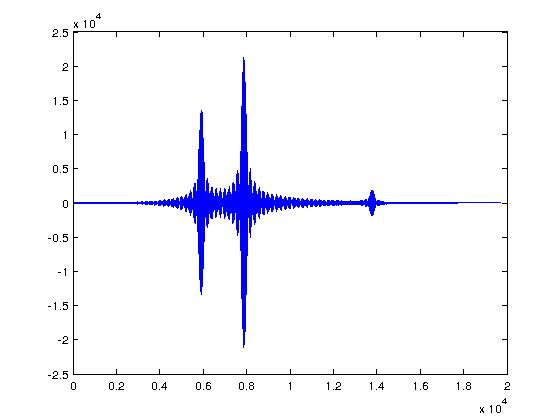
\includegraphics[height = 7.3 cm]{xsinc.jpg}
\caption{The function \eqref{eq:ex-signal}}
\label{fig:x}
\end{figure}

\begin{figure}[h]
\centering
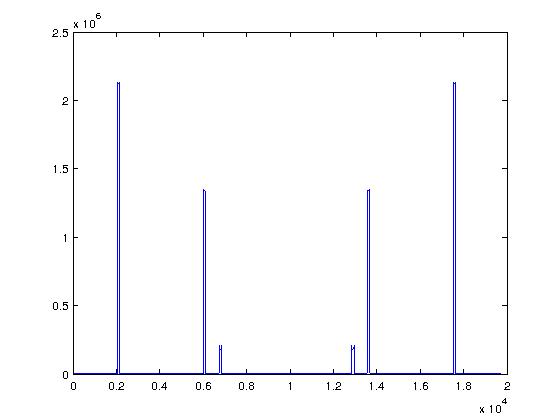
\includegraphics[height = 7.3 cm]{fftx.jpg}
\label{fig:fftx}
\caption{The fft of \eqref{eq:ex-signal}}
\end{figure}

In this case \(m = 50\) and \(L = 195\). Thie size of x \(= 19695\). The measurement system \eqref{eq:measurement} can be augmented to become:

\begin{equation}
y = \left(A \otimes I_{101}\right)x + n
\end{equation}

\bibliography{cswireless2}

\end{document}